\ifx\frameselection\somethingundefined
\def\frameselection{1-2}
\fi

\begin{saveblock}{basicDocCode}
    \begin{highlightblock}[linewidth=\textwidth,gobble=8]
        \title{My document}
        \author{Vincent Kuhlmann}
        \date{3 May 2021}
        
        \begin{document}
        \maketitle        
        \section{Lorem ipsum}
        Lorem ipsum dolor sit amet, consectetuer ...

        \begin{align}
            f(x) = \dfrac{1}{\sigma\sqrt{2\pi}} e^{
                -\frac{1}{2}\left(\frac{x-\mu}{\sigma}\right)^2}
        \end{align}
    \end{highlightblock}
\end{saveblock}
\ifx\frameselection\somethingundefined
\def\frameselection{1-}
\fi

\def\pasteframeselection#1{\begin{frame}<#1>}%
\expandafter\pasteframeselection\expandafter{\frameselection}%
\frametitle{\LaTeX{} vs Word}

\ifbool{english}{
    Inner workings: big difference.

    Word: Edit visually\\
    \LaTeX: Edit code (text)
}{
    Onder de motorkap: groot verschil.
    
    Word: Visueel, \LaTeX: Code (tekst).
}

\pause
\medskip

\begin{columns}[t]%
    \begin{column}{0.6\textwidth}
        \adjustbox{max height=0.6\textheight}{
            \useblock{basicDocCode}
        }
    \end{column}%
    \begin{column}{0.4\textwidth}%
        \adjustbox{fbox=0.5pt 0pt 0pt,margin=-30pt 0pt 0pt 0pt,set height=0pt}{%
            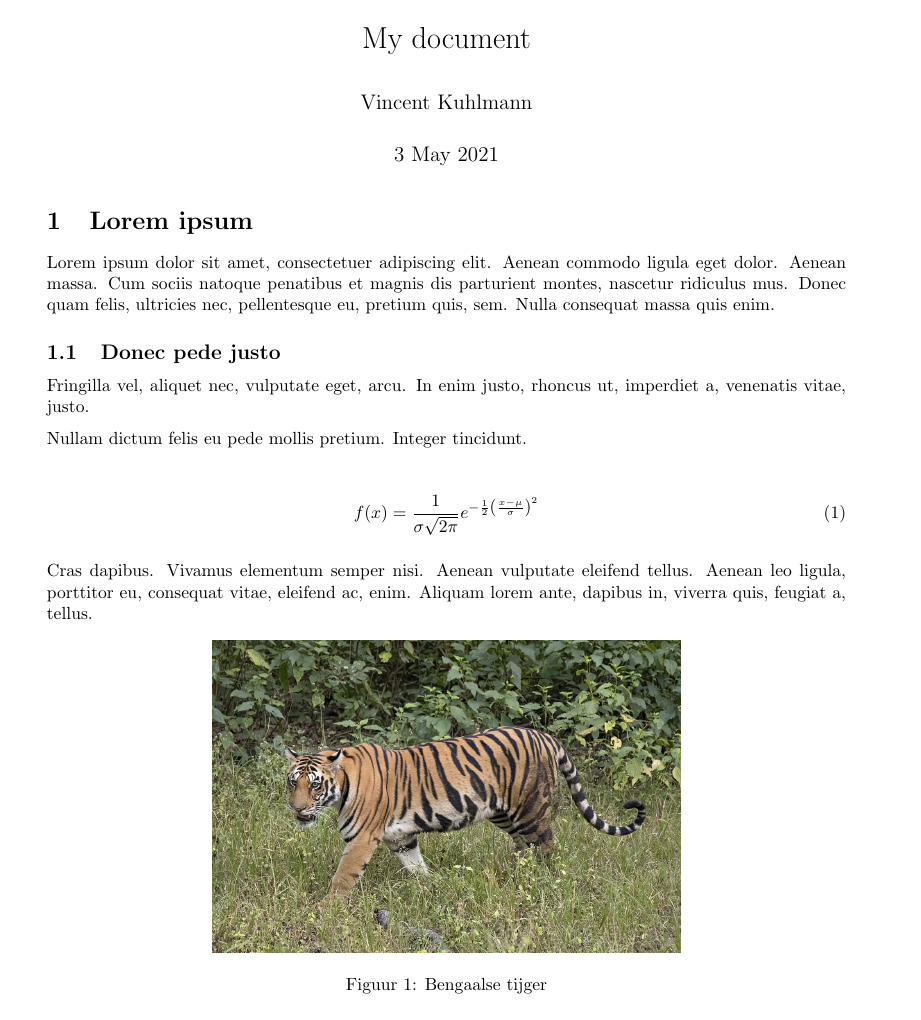
\includegraphics[width=1.6\linewidth,height=0.9\textheight,keepaspectratio]{assets/basicDocLaTeXSnippet.png}%
        }
    \end{column}%
\end{columns}
\end{frame}

\let\frameselection\somethingundefined
